\section{Empirical Evaluation}
\label{sec:evaluation}

\subsection{Validation}
\label{subsec:validation-with-counterfactual-data}

The validation process is structured in two phases

\paragraph{Initial validation}
In the initial phase, the generated expression is executed via Fluid CLI. If the execution is successful, the
result obtained is compared with the expected result. In case of error, the output is forwarded to the
\InterpretationAgent, which proceeds to regenerate the expression.

\paragraph{Validation via counterfactual testing}
In the second phase, the data used for execution is deliberately modified in order to verify the consistency
of the behaviours. Both the expected and generated expressions are executed again and the results are
compared. If discrepancies emerge, the error is forwarded to the \InterpretationAgent. If there are no
differences, the expression is considered valid and is returned to the user.

\subsection{Research questions}

These seem quite pertinent to the overall problem of transparent science communication:
\begin{itemize}
\item How does performance degrade with partial/ambiguous information?
\item How is performance affected by ``adversarial'' (intentionally/unintentionally misleading) information?
\end{itemize}

Some ways we might explore these axes:
\begin{itemize}
\item meaningful vs.~meaningless vs.~misleading identifiers
\item leaving out key criteria (e.g.~year) that would resolve query to unique answer
\end{itemize}

We might want to distinguish ambiguity inherent in the problem domain (e.g.~uncertainty) vs.~ambiguity in the
specification of a particular code-generation query.

\subsection{Success Rate by Category}
To evaluate the system we used a sample of the Scigen dataset~\citep{scigen_dataset_2021}.

We aggregated the generated expression in three categories: aggregation, trends, quantitative (See Table \ref{tab:fluid_examples}).
Figure \ref{fig:success_rate_by_category} shows the results obtained in generating expression by categories.

\begin{figure}
    \centering
    \begin{subfigure}{0.48\linewidth}
        \centering
        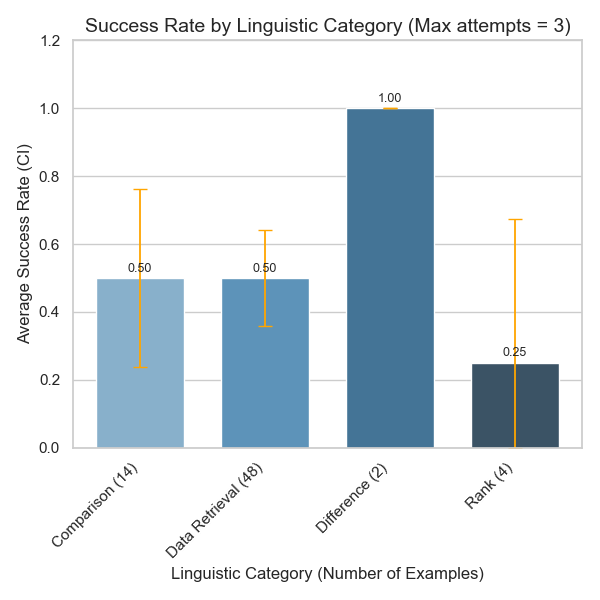
\includegraphics[width=\linewidth]{fig/success_rate_by_category}
        \caption{Success rate by testcases}
        \label{fig:success_rate_by_category}
    \end{subfigure}\hfill
    \begin{subfigure}{0.48\linewidth}
        \centering
        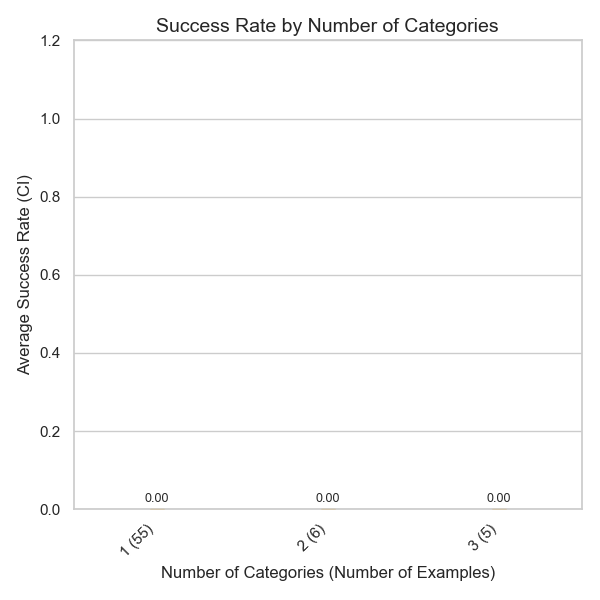
\includegraphics[width=\linewidth]{fig/success_rate_by_category_count}
        \caption{Success rate by category count}
        \label{fig:success_rate_by_category_count}
    \end{subfigure}
    \caption{Comparison of success rates}
    \label{fig:success_rate_comparison}
\end{figure}


\subsection{Negative Cases}
\label{subsec:negative-cases}

\begin{table}[t]
    \centering
    \small
    \begin{tabular}{l p{6cm} p{4cm}}
        \hline
        \textbf{Problem Type} & \textbf{Example} & \textbf{Explanation} \\
        \hline

        ambiguous referent &
        As shown in Table 3 \hl{BiLSTM} gives significantly better accuracies compared to uni-directional LSTM with the training time per epoch growing from 99 seconds to 106 seconds &
        There are three models that have 99 seconds as their time; the assistant would not know which one to choose. \\

        missing data &
        The average methane emissions for the year 2015 is \hl{1.0} &
        November is missing to calculate the average correctly. \\

        false statement &
        We additionally make comparisons with stacked CNNs and hierarchical attention (Vaswani et al., 2017), shown in Table 3 (the CNN and Transformer rows), BiLSTM is \hl{the most efficient} among all models compared, with the highest model size &
        BiLSTM is not the most efficient, nor does it have the largest size. \\

        incorrect numerical value &
        LSTM is the fastest model with overall time taken being \hl{90} seconds &
        It is not 90 but 106. \\

        ambiguous referent &
        LSTM is the fastest model with overall time taken being \hl{90} seconds &
        There are two type of time in the dataset (training\_time, execution\_time), both with a value of 90 seconds. \\

        \hline
    \end{tabular}
    \caption{Categories of problematic example}
    \label{tab:ambiguita}
\end{table}





